\documentclass[a4paper,11pt]{article}
\usepackage{lmodern}
\renewcommand*\familydefault{\sfdefault}
\usepackage{sfmath}
\usepackage[utf8]{inputenc}
\usepackage[T1]{fontenc}
\usepackage[italian]{babel}
\usepackage{indentfirst}
\usepackage{graphicx}
\usepackage{tikz}
\newcommand*\circled[1]{\tikz[baseline=(char.base)]{
            \node[shape=circle,draw,inner sep=2pt] (char) {#1};}}
\usepackage{enumitem}
% \usepackage[group-separator={\,}]{siunitx}
\usepackage[left=2cm, right=2cm, bottom=3cm]{geometry}
\frenchspacing

\newcommand{\num}[1]{#1}

% Macro varie...
\newcommand{\file}[1]{\texttt{#1}}
\renewcommand{\arraystretch}{1.3}
\newcommand{\esempio}[2]{
\noindent\begin{minipage}{\textwidth}
\begin{tabular}{|p{11cm}|p{5cm}|}
    \hline
    \textbf{File \file{input.txt}} & \textbf{File \file{output.txt}}\\
    \hline
    \tt \small #1 &
    \tt \small #2 \\
    \hline
\end{tabular}
\end{minipage}
}

% Dati del task
\newcommand{\gara}{Olimpiadi Italiane di Informatica -- Salerno 2013}
\newcommand{\nome}{Maree a Venezia}
\newcommand{\nomebreve}{maree}

\begin{document}
% Intestazione
\noindent{\Large \gara}
\vspace{0.5cm}

\noindent{\Huge \textbf \nome~(\texttt{\nomebreve})}

% Descrizione del task
\section*{Descrizione del problema}
I gondolieri di Venezia si spostano lungo i canali, seguendo la
corrente. Ogni canale è quindi percorribile in una sola direzione,
nota ai gondolieri. Quando però arriva l'alta marea, le dinamiche
della laguna sono tali che il verso della corrente di ogni canale si
inverte. Dovete aiutare i gondolieri a pianificare il loro percorso
per spostarsi in gondola da un punto di origine a un punto di
destinazione, sapendo che sta per arrivare l'alta marea.

Data la mappa degli $N$ punti di intersezione e degli $M$ canali della città di Venezia che li collegano, con le correnti che inizialmente
ne fluiscono, dovete determinare il minimo tempo necessario per spostarsi in gondola dal punto $0$ al punto $N-1$,
tenendo presente che:
\begin{itemize}
\item per attraversare un canale -- cosa possibile solo nel senso della corrente -- si impiega esattamente 1 minuto;
\item dopo $T$ minuti arriva l'alta marea e quindi la direzione di percorrenza di tutti i canali si inverte;
\item nei punti di intersezione di due o più canali è possibile fermarsi per un numero di minuti a piacere.
\end{itemize}

\begin{center}
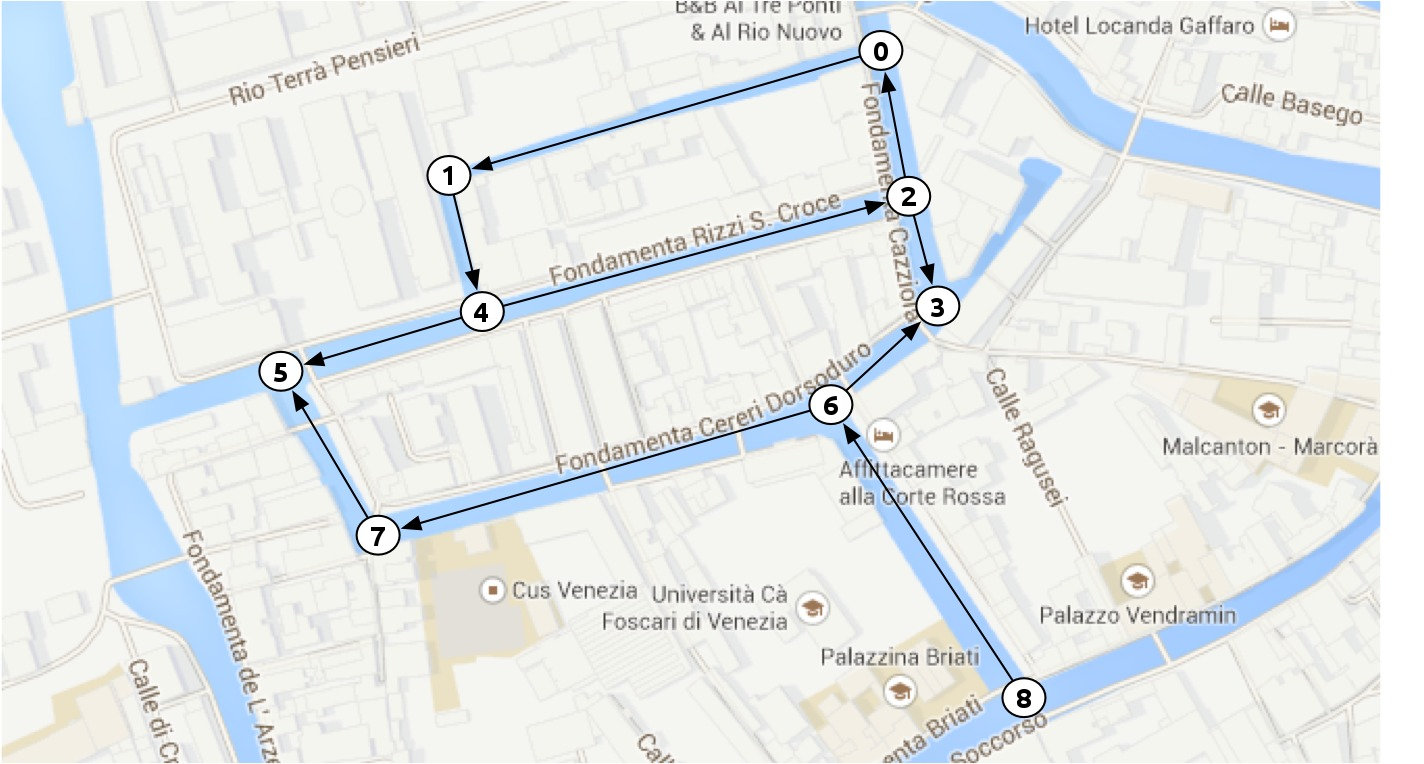
\includegraphics[width=13cm]{maree.jpg}
\end{center}

Per esempio, considerate questa mappa. Per andare dal punto $0$
al punto $N-1 = 8$, sapendo che l'alta marea arriverà al minuto $T=5$,
si può seguire il seguente percorso (che richiede 7 minuti):
\begin{itemize}[nolistsep,noitemsep]
\item da $t=0$ a $t=1$: $\circled 0 \to \circled 1$
\item da $t=1$ a $t=2$: $\circled 1 \to \circled 4$
\item da $t=2$ a $t=3$: $\circled 4 \to \circled 2$
\item da $t=3$ a $t=4$: $\circled 2 \to \circled 3$
\item da $t=4$ a $t=5$: si rimane fermi in $\circled 3$
\item in $t=5$: alta marea
\item da $t=5$ a $t=6$: $\circled 3 \to \circled 6$
\item da $t=6$ a $t=7$: $\circled 6 \to \circled 8$
\end{itemize}

Un percorso alternativo, sebbene richieda 8 minuti e quindi non sia una soluzione valida, è il seguente:
\begin{itemize}[nolistsep,noitemsep]
\item da $t=0$ a $t=1$: $\circled 0 \to \circled 1$
\item da $t=1$ a $t=2$: $\circled 1 \to \circled 4$
\item da $t=2$ a $t=3$: $\circled 4 \to \circled 5$
\item da $t=3$ a $t=5$: si rimane fermi in $\circled 5$
\item in $t=5$: alta marea
\item da $t=5$ a $t=6$: $\circled 5 \to \circled 7$
\item da $t=6$ a $t=7$: $\circled 7 \to \circled 6$
\item da $t=7$ a $t=8$: $\circled 6 \to \circled 8$
\end{itemize}

\`E facile verificare che, nella mappa mostrata, non ci sono modi di
arrivare in $N-1$ in meno di 7 minuti.

Per risolvere il problema,
dovete scrivere una funzione $\texttt{solve} (N, M, T, S, E)$, che
restituisca un singolo numero intero: il minimo tempo necessario per
arrivare dal punto $0$ al punto $N-1$, sapendo che l'$i$-esimo degli
$M$ canali collega i punti di intersezione $S_i$ ed $E_i$, che la
corrente inizialmente fluisce da $S_i$ a $E_i$, e che l'alta marea
arriva al minuto $T$.  Se non è possibile andare dal punto $0$ al
punto $N-1$, allora la funzione deve restituire il valore $-1$.

% Subtask
\section*{Subtask}
\begin{itemize}
\item \textbf{Subtask 0 \phantom{1}[5 punti]:} caso di esempio.
\item \textbf{Subtask 1 [11 punti]:} $2 \le N\le 100\,000$, $1 \le M\le 2\,000\,000$ e $T = 0$.
\item \textbf{Subtask 2 [25 punti]:} $2 \le N \le 3\,000$, $1 \le M \le 20\,000$ e $0 \le T \le 1\,000\,000\,000$.
\item \textbf{Subtask 3 [38 punti]:} $2 \le N \le 100\,000$, $1 \le M\le 2\,000\,000$ e $0 \le T \le 1\,000\,000\,000$.
\item \textbf{Subtask 4 [21 punti]:} $2 \le N \le 200\,000$, $1 \le M \le 3\,000\,000$ e $0 \le T \le 1\,000\,000\,000$.
\end{itemize}

% Implementazione

\section*{Dettagli di implementazione}
Dovrai sottoporre esattamente un file con estensione: \texttt{.c},
\texttt{.cpp} o \texttt{.pas}. Questo file deve implementare la
funzione $\texttt{solve}$ utilizzando uno dei seguenti
prototipi.

\subsection*{Programma in C o C++}
\begin{verbatim}
int solve(int N, int M, int T, int* S, int* E);
\end{verbatim}

\subsection*{Programma in Pascal}
\begin{verbatim}
function solve(N, M, T: longint; var S, E: array of longint): longint;
\end{verbatim}

La funzione implementata dovrà comportarsi come sopra
descritto. Naturalmente sei libero di implementare altre routine
ausiliarie per uso interno. La tua sottoposizione non deve effettuare
direttamente operazioni di input o output, via console o via file di
testo.

\subsection*{Funzionamento del grader di esempio}
Nella directory relativa a questo problema è presente una versione
semplificata del grader usato durante la correzione, che potete usare
per testare le vostre soluzioni in locale. Il grader di esempio legge
i dati di input dal file \file{input.txt}, chiama la funzione che
dovete implementare, e scrive il risultato restituito dalla vostra
funzione sul file \file{output.txt}. Il file \file{input.txt} deve
essere composto da $M+1$ righe, in questo formato:
\begin{itemize}
\item nella prima riga devono essere presenti 3 interi: $N$, $M$, $T$;
\item nella $i$-esima delle successive $M$ righe devono essere presenti 2 interi: $S_i$ e $E_i$.
\end{itemize}


% Esempi
\section*{Esempio di input/output}

\esempio{
9 10 5

0 1

1 4

4 2

2 0

2 3

4 5

7 5

6 7

6 3

8 6
}{7}


Nota: l'esempio riportato è relativo alla situazione mostrata in figura.

\end{document}
